\section{MPI One-Sided Communication}
\subsection{Required submission files}
\begin{enumerate}
  \item \hl{The updated \emph{gauss.c} file.}

    \verb!Data/one_sided/gauss.c!

  \item \hl{The new performance plots and description in the report.}

	Please refer to the following Fig \ref{fig:compute_multdomain_os_baseline}, \ref{fig:mpi_multdomain_os_baseline}, \ref{fig:total_multdomain_os_baseline}, \ref{fig:compute_multdomain_os_nb}, \ref{fig:mpi_multdomain_os_nb}, \ref{fig:total_multdomain_os_nb}. The vampir plot is Fig. \ref{fig:vampir_haswell_one_sided}.

\end{enumerate}

\subsection{Questions}
\begin{enumerate}
  \item \hl{Which one-sided operations were used? Justify your choice.}

	We targeted the blocking \verb!MPI_Send! and \verb!MPI_Recv! functions passing pivot data for optimization.
	These were the most affected by the blocking operations and were the most likely to benefit from overlapping communication and computation.
    We decided to use the Post-Start-Wait-Complete methodology, which uses the following 
    MPI functions: \verb!MPI_Win_start!, \verb!MPI_Win_post!, \verb!MPI_Win_wait!, \verb!MPI_Win_complete!, and \verb!MPI_Win_get!. 
    This methodology allows the use of unique MPI communication groups---specifying the specific processes which are allowed to participate in a particular exposure/access epoch.
    This is useful for this use case as the communication of information only goes from processes with a lower rank number to processes with a higher rank number when distributing the pivot data.
    There is additionally a final aggregation phase where the computed information is passed back to process 0.
    However, the time associated with this phase is negligible in relation to the time spent communicating pivot data.
    We have decided to go with \verb!MPI_Get! function because it fits the purpose of distributing
    data from the process that had computed his part of pivoting to the rest.

  \item \hl{Was communication and computation overlap achieved? Use Vampir.}

    No, this was not achieved. 
    The execution of the program is purely sequential because the no computation occurs during communication.
    No computation occured during the exposure or the access epochs.
    This can be seen from Fig. \ref{fig:vampir_haswell_one_sided}.
    The applied code should reduce the sequential nature of the sends and receives, such that multiple sends and receives can take place concurrently.
    \begin{figure}[h] % h=here, t=top, b=bottom, p=(extra)page, !=force
	\begin{center}
			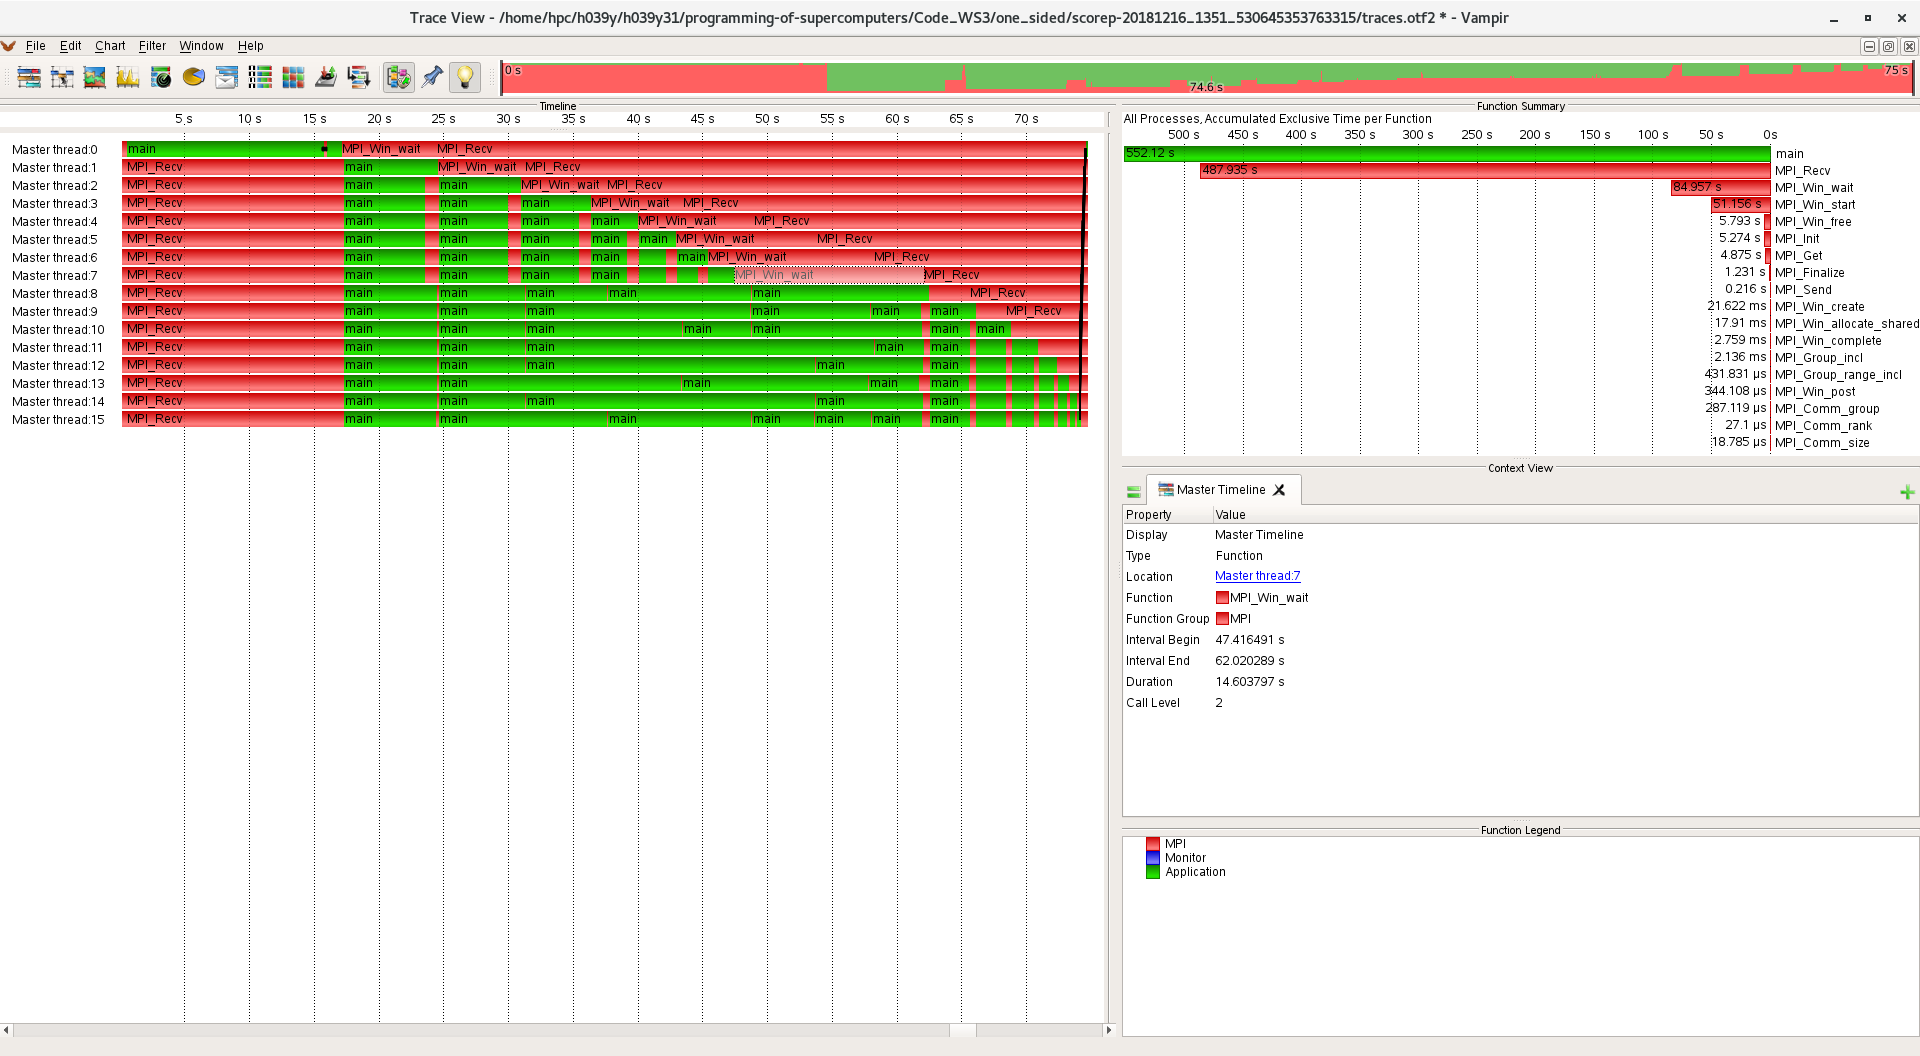
\includegraphics[width=.8\linewidth]{/one_sided/vampir_onesided_hw.png}
		\caption{Vampir output for One-Sided Communication, Haswell}
		\label{fig:vampir_haswell_one_sided}
	\end{center}
	\end{figure}
	

  \item \hl{Was a speedup observed versus the baseline for the Sandy Bridge and Haswell nodes?}

    Results performed on Haswell and Sandy Bridge for one-sided communication are similar.
  
    Despite the implementation of the one-sided communication, overall time was general worse than
    that for baseline. 
    This was due the fact that processors with a higher rank number had longer computation times. 
    Therefore, they become a bottleneck for this implementation. 
    
    We can view the results comparing the computational time and MPI time of the Baseline and the One-Sided communication below. 
    
    When comparing the compute times for the baseline and one-sided communication. We see that the baseline implementation is generally faster.
    This is true for most domains, as can be seen in Fig. \ref{fig:compute_multdomain_os_baseline}.
    However, we also see that the one-sided implementation is faster for certain combinations of domain size and process counts.
    This is true, for Haswell nodes with a domain size of 4096, we see that the one-sided communication has a slightly shorted compute time.
    This general trend is not seen for Sandy Bridge nodes, and compute times are overall slower when comparing the two implementations. 
    
    	\begin{figure}[h] % h=here, t=top, b=bottom, p=(extra)page, !=force
		\hspace*{-0.25\linewidth}\begin{tabular}{cc}
			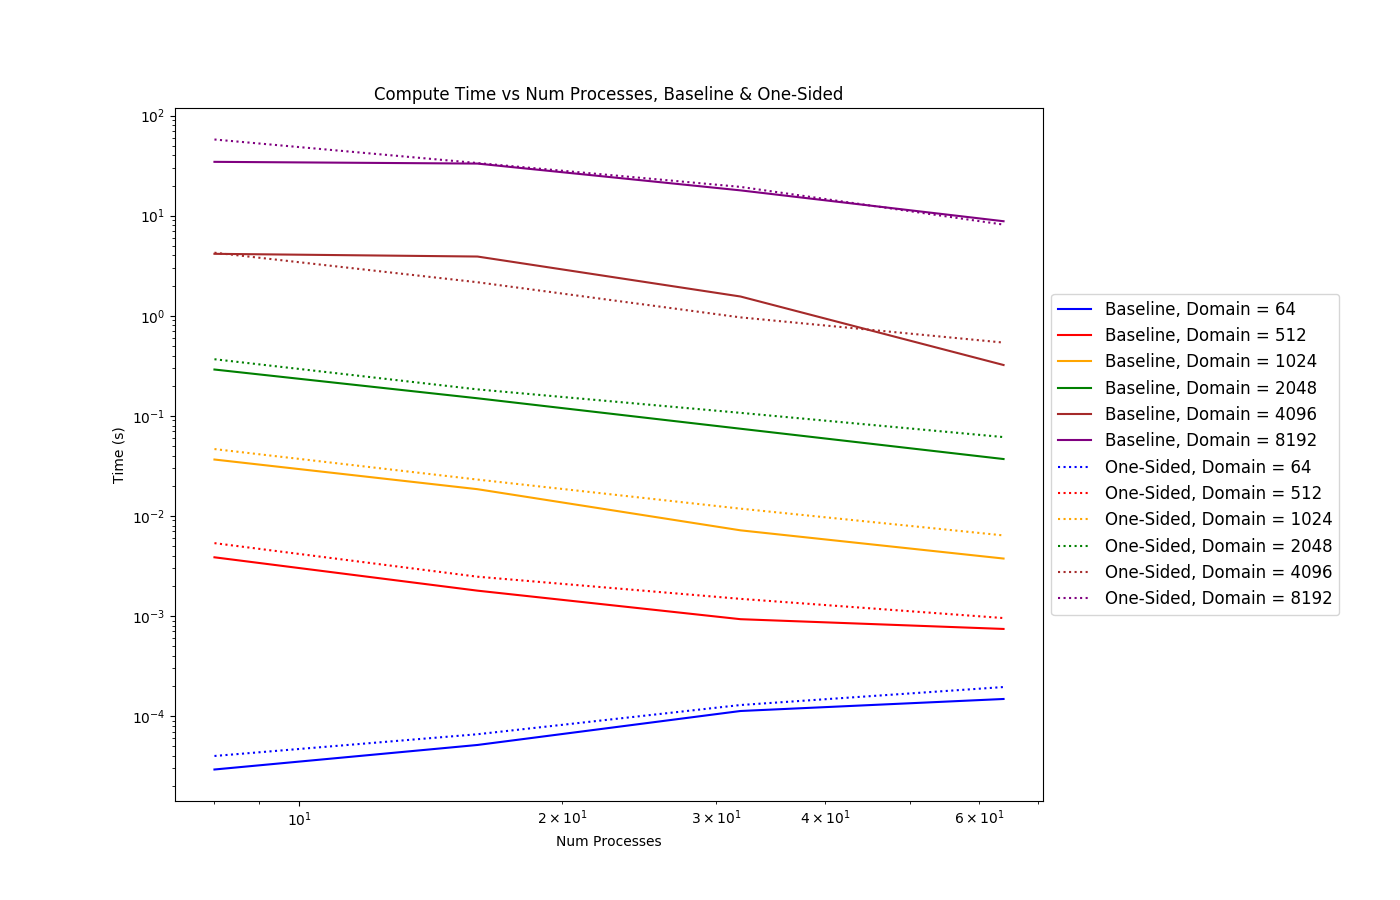
\includegraphics[width=.75\linewidth]{one_sided/compute_multdomain_haswell_os_baseline.png} & 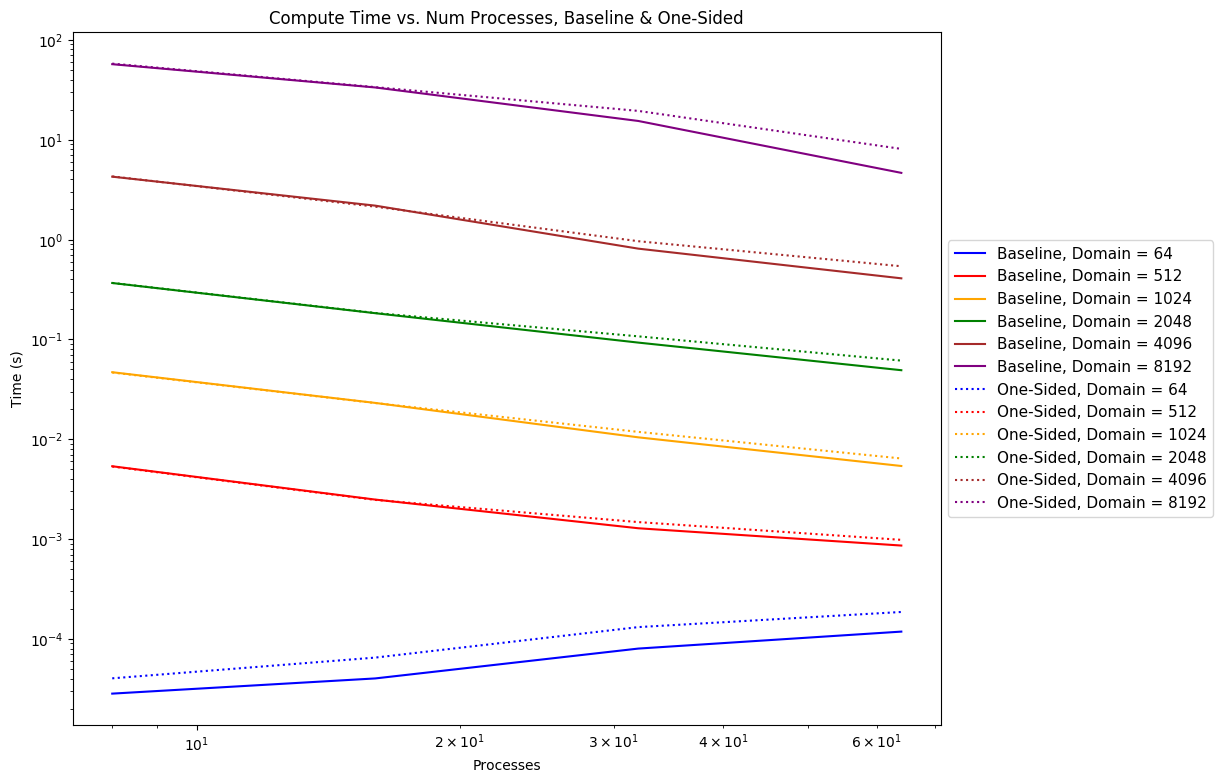
\includegraphics[width=.75\linewidth]{one_sided/compute_multdomain_sandy_os_baseline.png} \\
			(a) Haswell &  (b) Sandy Bridge\\[6pt]
		\end{tabular}
		\caption{Compute Time vs. \#Processes., One-Sided vs. Baseline}
		\label{fig:compute_multdomain_os_baseline}
	\end{figure}
	When comparing the MPI times for the baseline and the one-sided implentation, the baseline is generally faster. 
	However, for certain combinations of domain size and process counts, the non-blocking implementation is faster. 
	This is generally true when the domain size is 4096 and for higher process counts at small domain sizes for Haswell nodes, as seen in Fig. \ref{fig:mpi_multdomain_os_baseline}.
		\begin{figure}[h] % h=here, t=top, b=bottom, p=(extra)page, !=force
		\hspace*{-0.25\linewidth}\begin{tabular}{cc}
			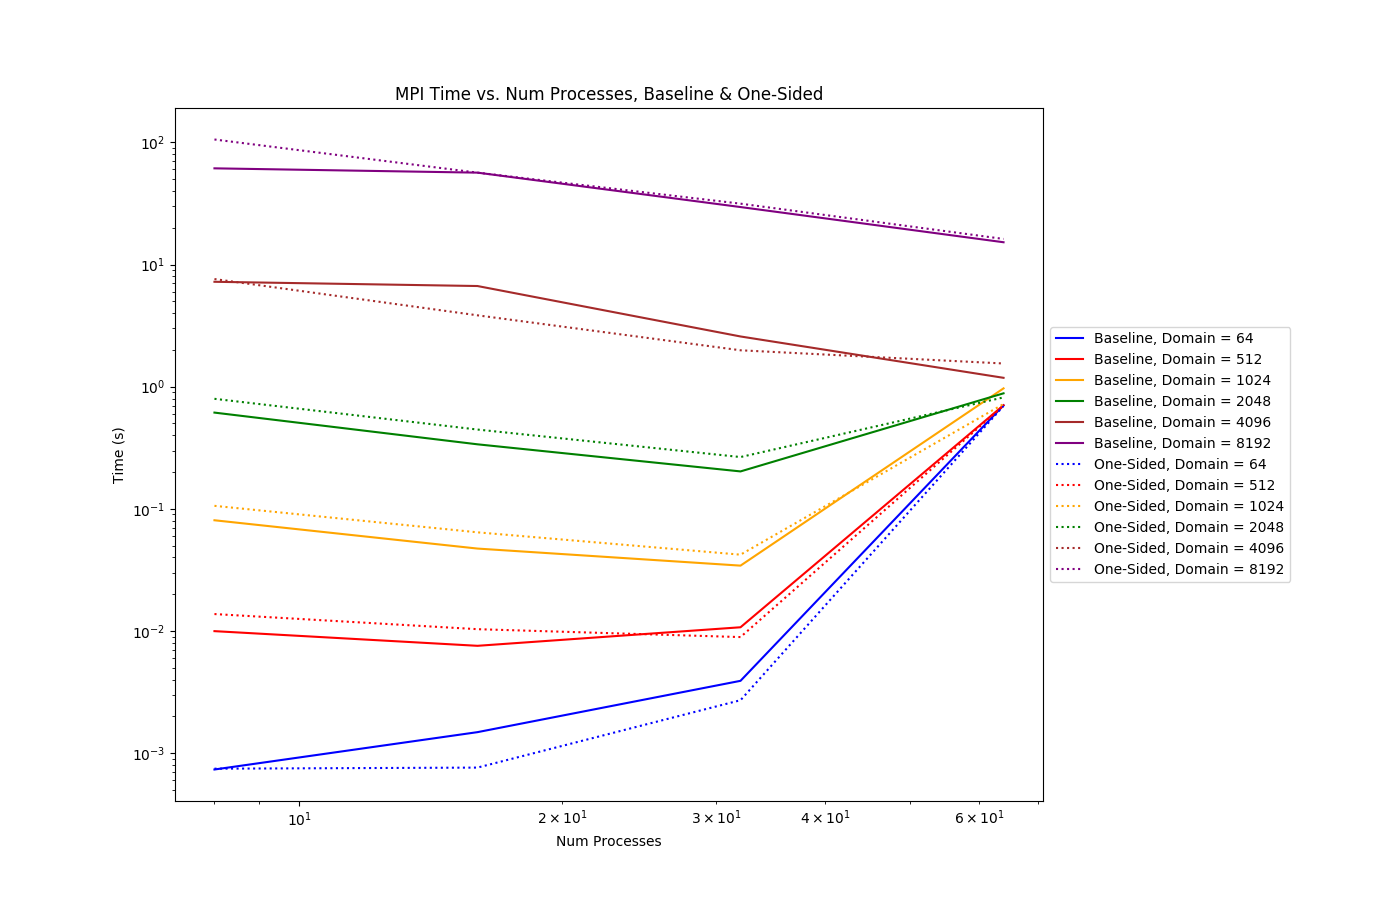
\includegraphics[width=.8\linewidth]{one_sided/mpi_multdomain_haswell_os_baseline.png} &
			 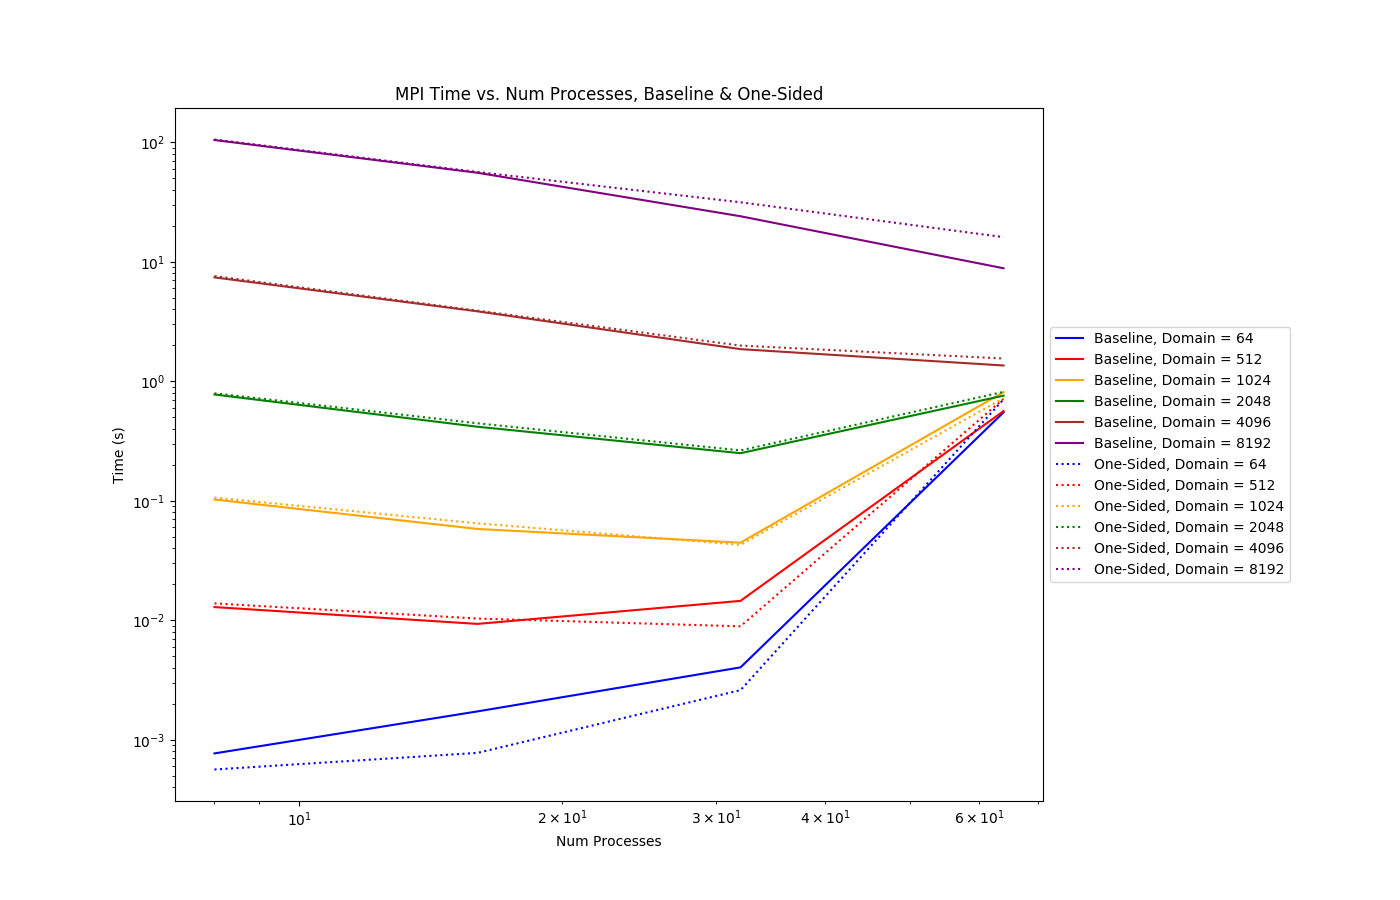
\includegraphics[width=.8\linewidth]{one_sided/mpi_multdomain_sandy_os_baseline.png} \\
			(a) Haswell &  (b) Sandy Bridge\\[6pt]
		\end{tabular}
		\caption{MPI Time vs. \#Processes., One-Sided vs. Baseline}
		\label{fig:mpi_multdomain_os_baseline}
	\end{figure}
	Similar trends are seen when comparing the total time of the two implementations, which is shown in Fig. \ref{fig:total_multdomain_os_baseline}. 	
			\begin{figure}[h] % h=here, t=top, b=bottom, p=(extra)page, !=force
		\hspace*{-0.25\linewidth}\begin{tabular}{cc}
			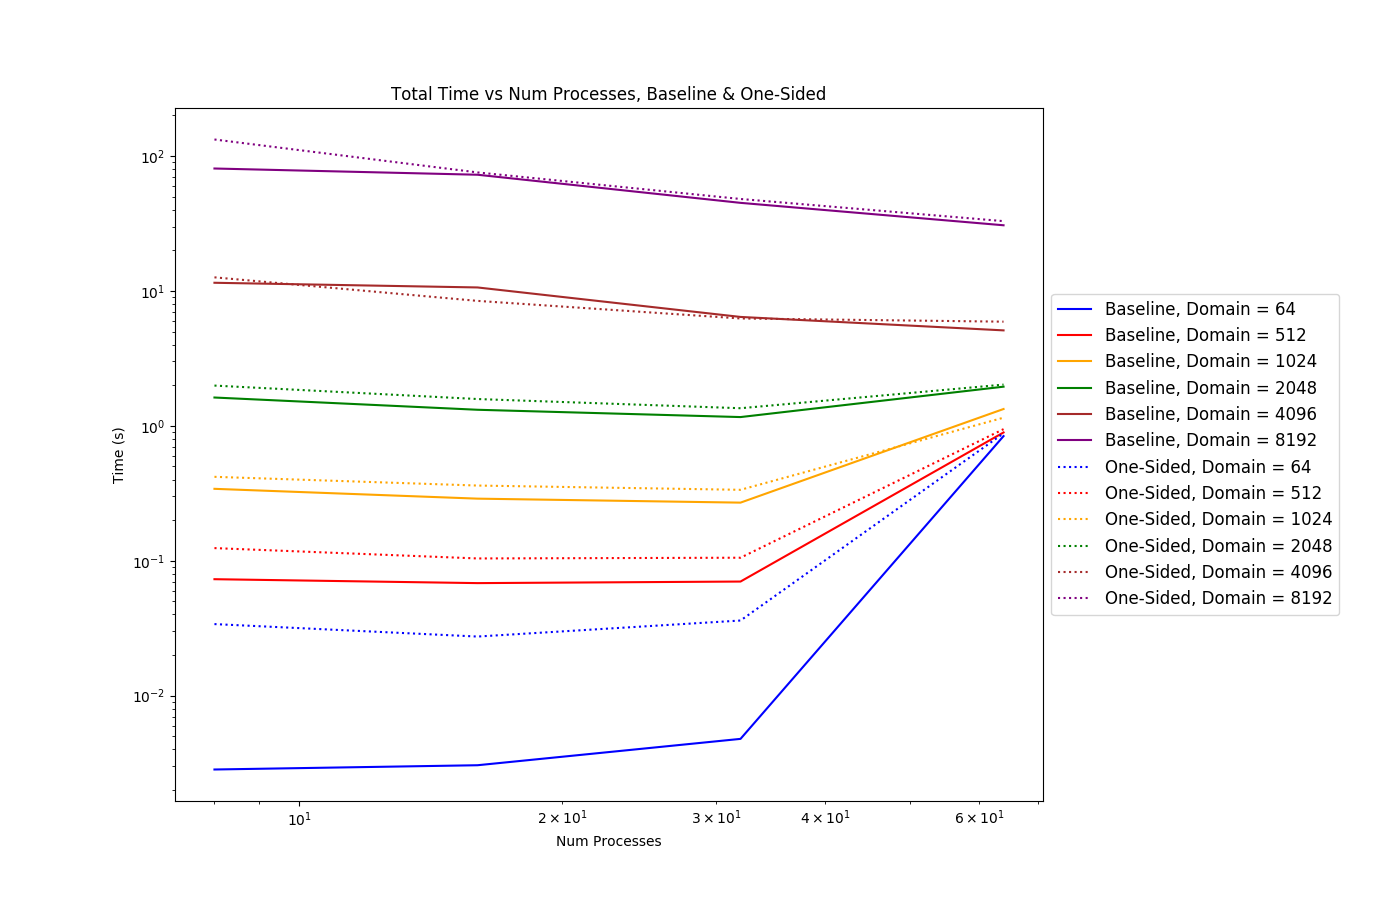
\includegraphics[width=.8\linewidth]{one_sided/total_multdomain_haswell_os_baseline.png} &
			 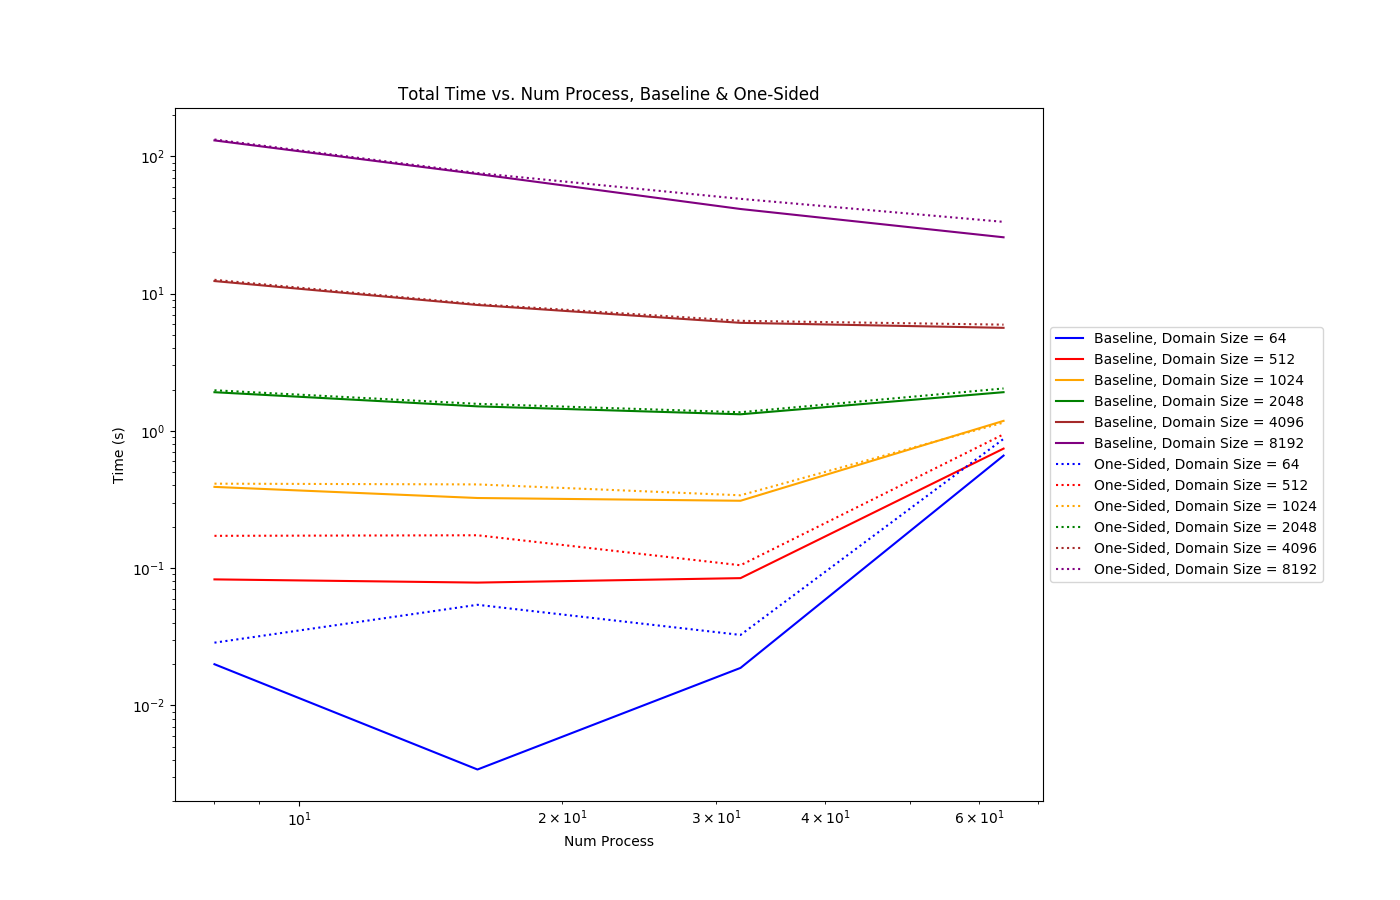
\includegraphics[width=.8\linewidth]{one_sided/total_multdomain_sandy_os_baseline.png} \\
			(a) Haswell &  (b) Sandy Bridge\\[6pt]
		\end{tabular}
		\caption{Total Time vs. \#Processes., One-Sided vs. Baseline}
		\label{fig:total_multdomain_os_baseline}
	\end{figure}
	
	Theoretically, we are be able to overlap communication and computation. However, this comes with the cost of additional synchronization. The optimal of combination both is very case specific. This would be done by splitting the local number of rows into chunks and interleaving communication and computation. However, finding the optimal chunk size is extremely task-specific optimization.

  \item \hl{Was a speedup observed versus the non-blocking version for the Sandy Bridge and Haswell nodes?}

	There was little speedup when comparing with the non-blocking version. Due to the inherent sequential nature of the communication. The non-blocking more consistently performed better than the one-sided communication. We can compare these results in the following plots.
	
	We can compare the compute times of the two implementations. Generally, the compute times are shorter for the non-blocking communication. 
	We do see that the non-blocking is slightly faster for certain domain sizes for both Haswell and Sandy bridge nodes, as seen in Fig. \ref{fig:compute_multdomain_os_nb}.
	    	\begin{figure}[h] % h=here, t=top, b=bottom, p=(extra)page, !=force
		\hspace*{-0.25\linewidth}\begin{tabular}{cc}
			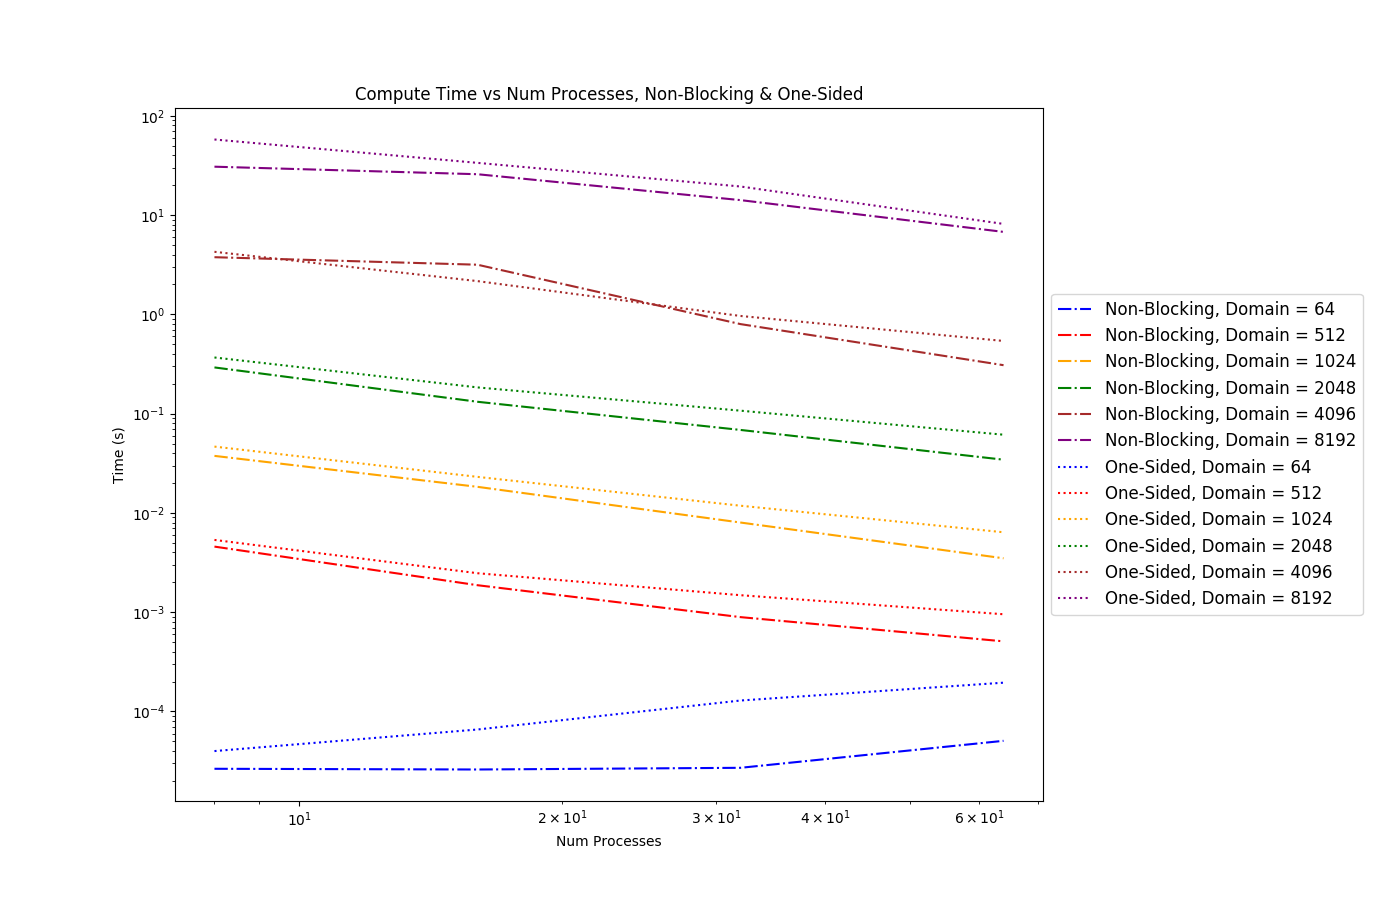
\includegraphics[width=.75\linewidth]{one_sided/compute_multdomain_haswell_os_nb.png} & 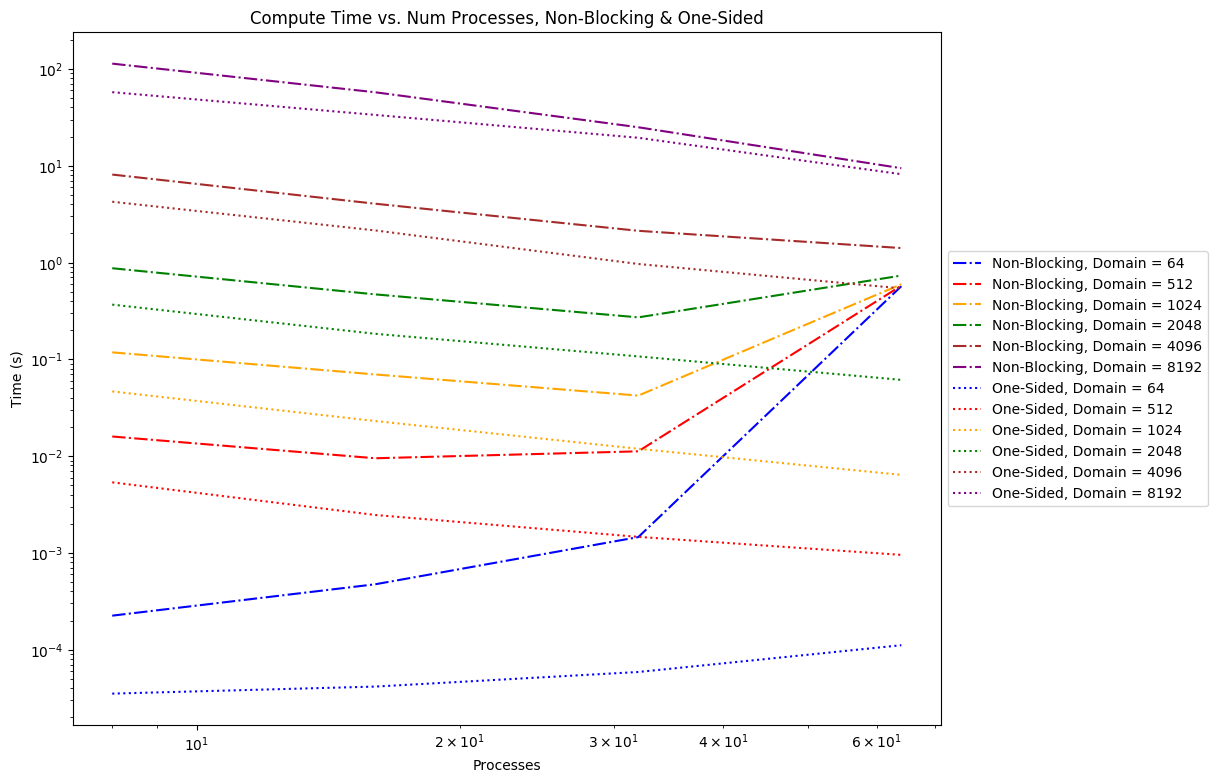
\includegraphics[width=.75\linewidth]{one_sided/compute_multdomain_sandy_os_nb.png} \\
			(a) Haswell &  (b) Sandy Bridge\\[6pt]
		\end{tabular}
		\caption{Compute Time vs. \#Processes., One-Sided vs Non-Blocking}
		\label{fig:compute_multdomain_os_nb}
	\end{figure}
	
	
	\begin{figure}[h] % h=here, t=top, b=bottom, p=(extra)page, !=force
		\hspace*{-0.25\linewidth}\begin{tabular}{cc}
			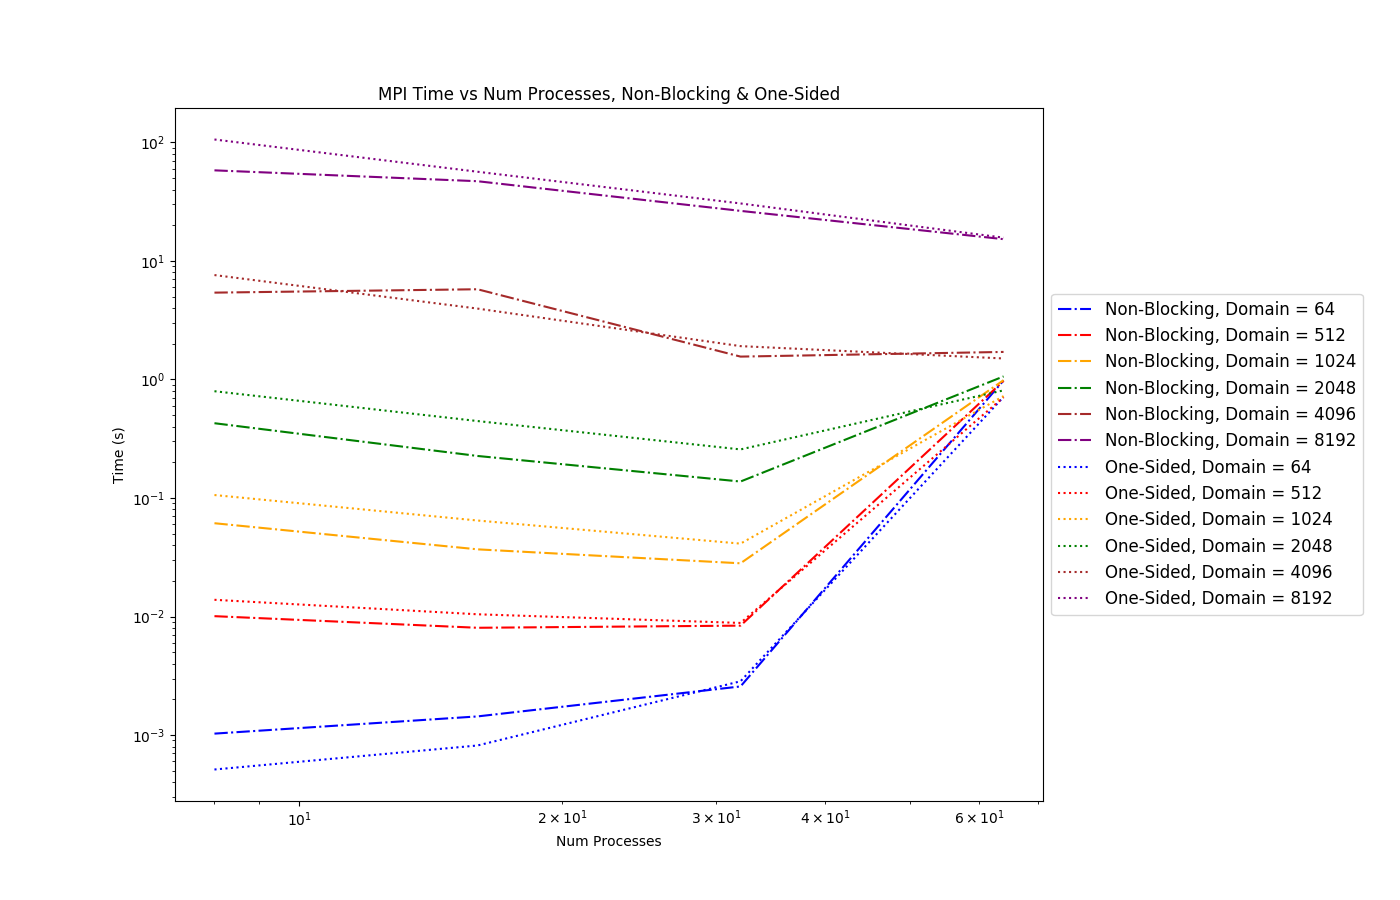
\includegraphics[width=.75\linewidth]{one_sided/mpi_multdomain_haswell_os_nb.png} & 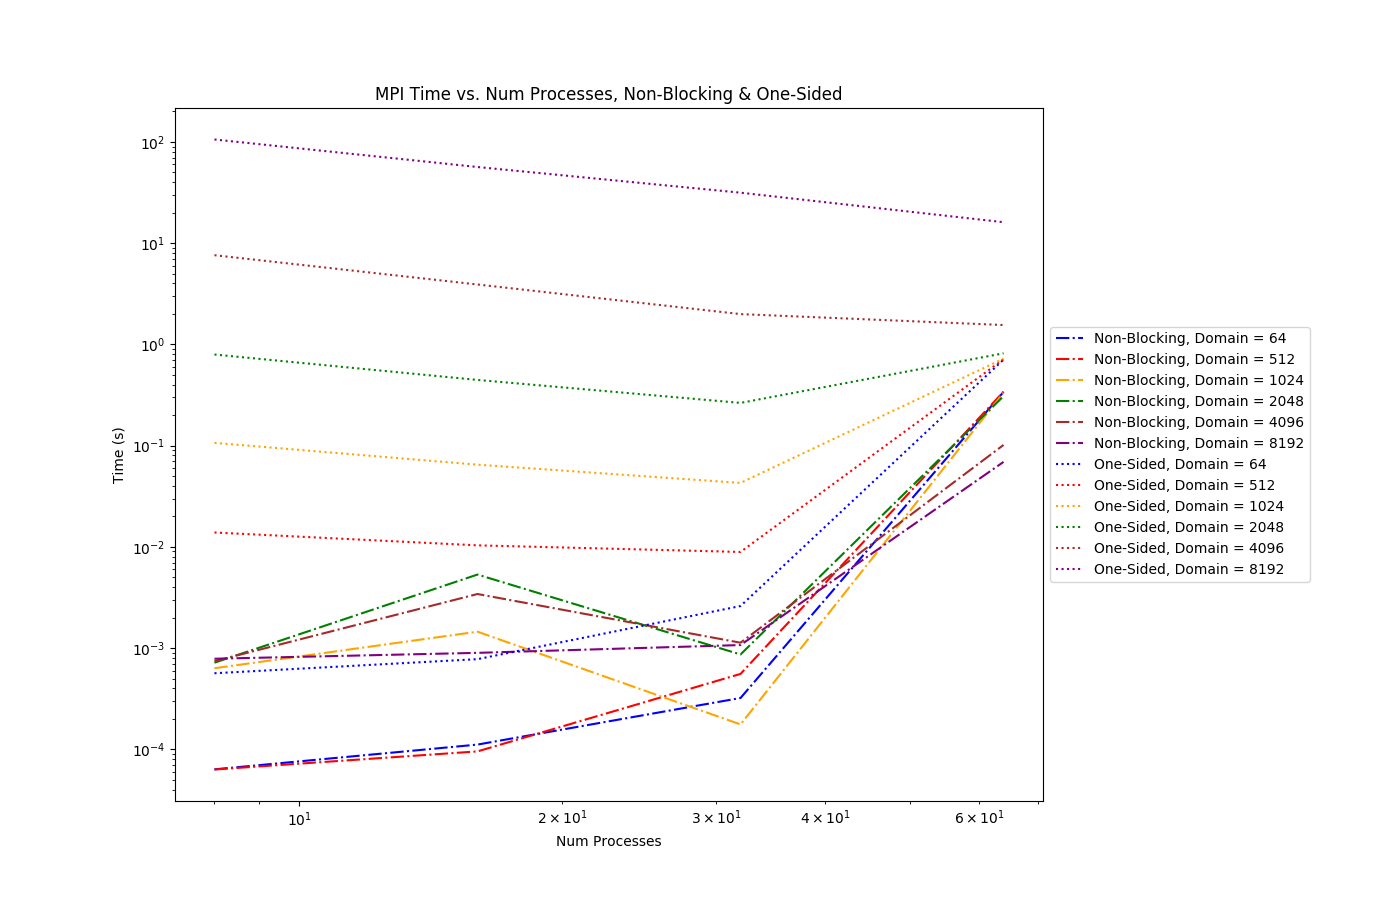
\includegraphics[width=.75\linewidth]{one_sided/mpi_multdomain_sandy_os_nb.png} \\
			(a) Haswell &  (b) Sandy Bridge\\[6pt]
		\end{tabular}
		\caption{MPI Time vs. \#Processes., One-Sided vs Non-Blocking}
		\label{fig:mpi_multdomain_os_nb}
	\end{figure}
	
	We see similar trends in MPI times, that the Haswell nodes are generally slightly slower. 
	However, interestingly, we see that the non-blocking performs generally better when the process count is increased to 64---for both Sandy Bridge and Haswell nodes, this is see in Fig. \ref{fig:mpi_multdomain_os_nb}.
			\begin{figure}[h] % h=here, t=top, b=bottom, p=(extra)page, !=force
		\hspace*{-0.25\linewidth}\begin{tabular}{cc}
			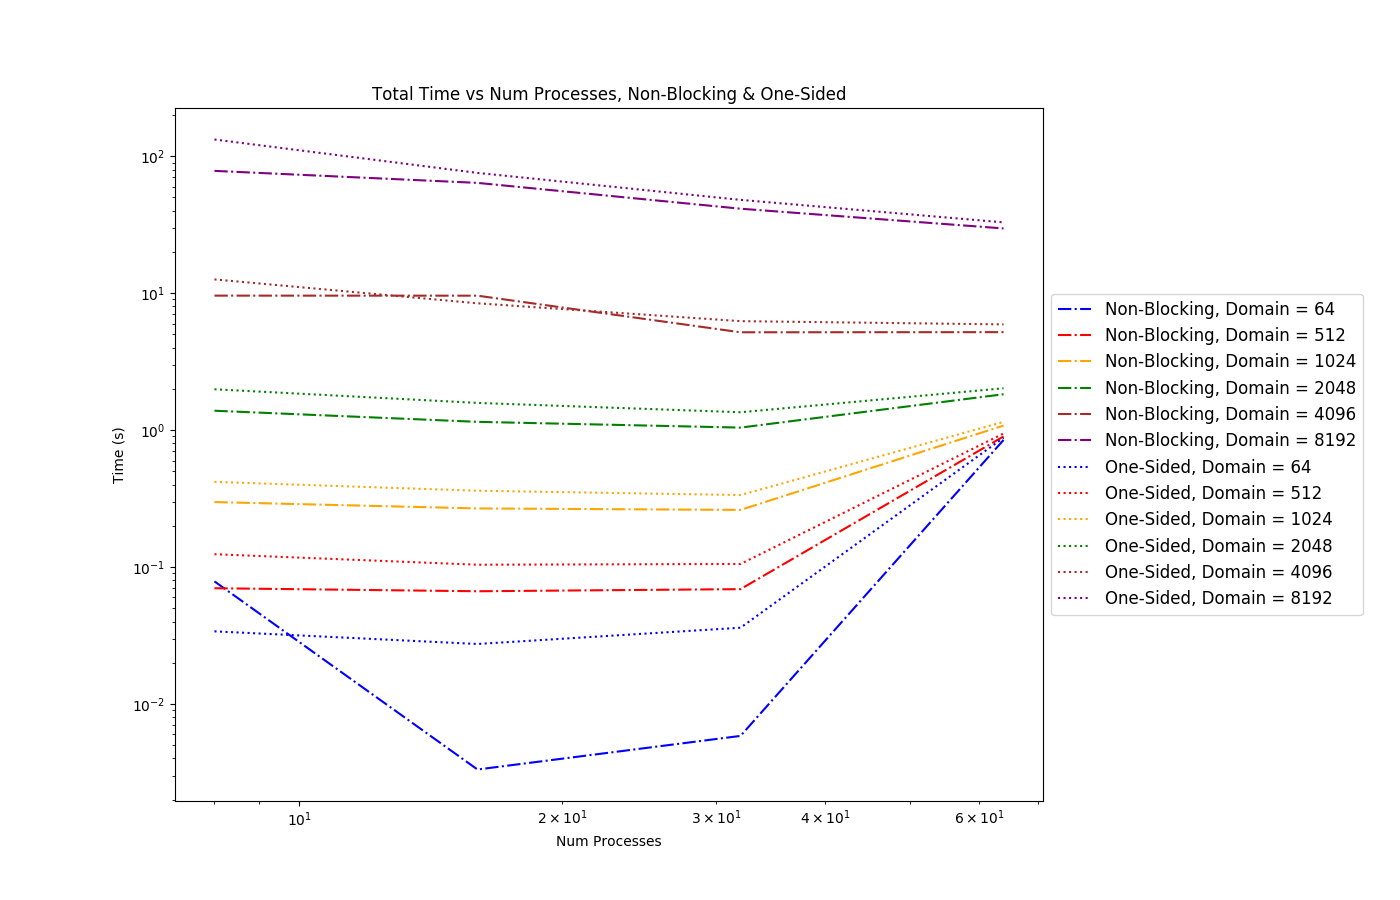
\includegraphics[width=.8\linewidth]{one_sided/total_multdomain_haswell_os_nb.png} & 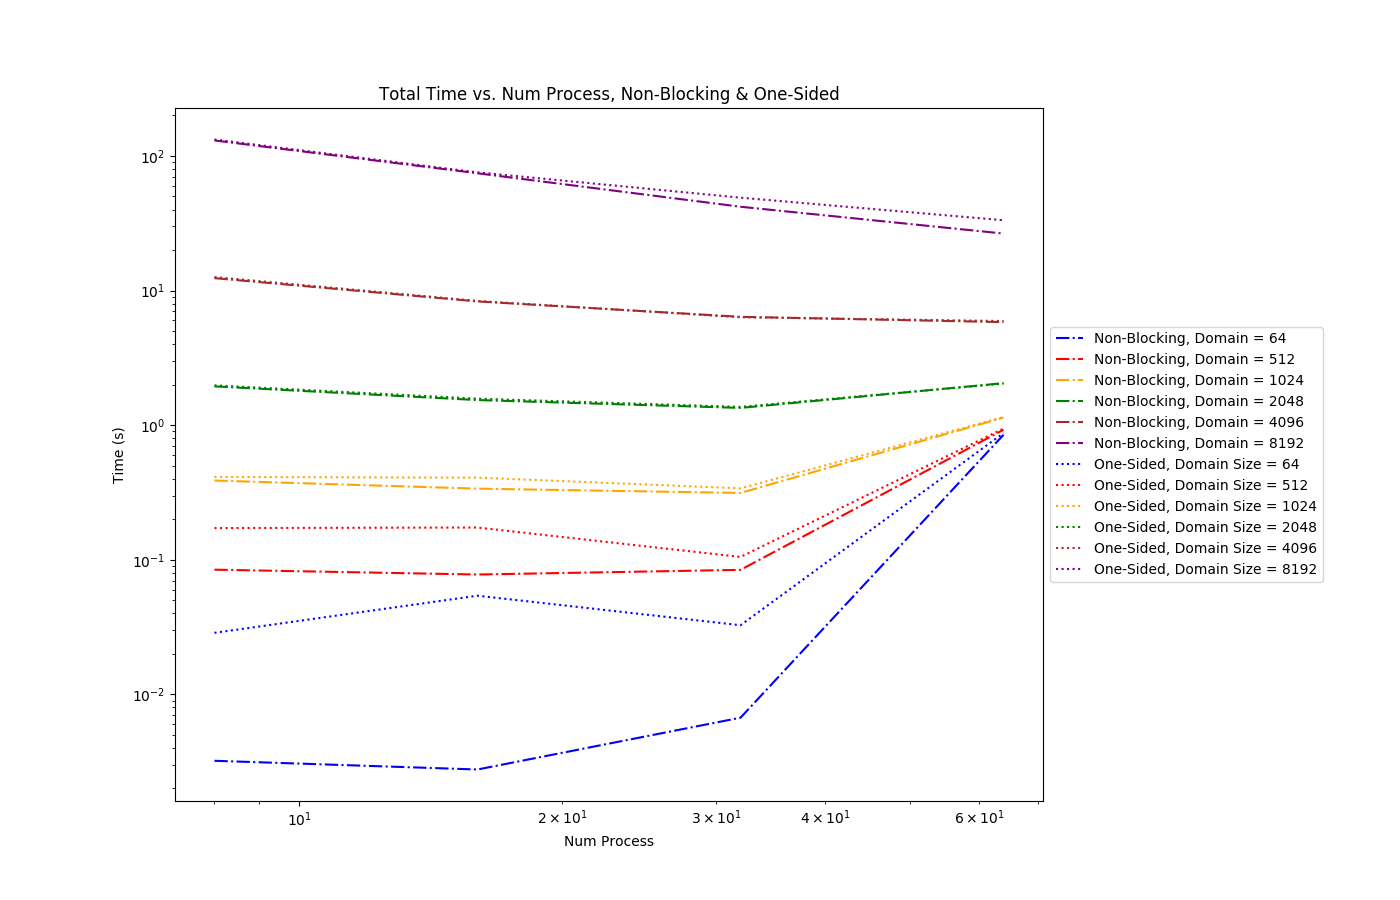
\includegraphics[width=.8\linewidth]{one_sided/total_multdomain_sandy_os_nb.png} \\
			(a) Haswell &  (b) Sandy Bridge\\[6pt]
		\end{tabular}
		\caption{Total Time vs. \#Processes., One-Sided vs. Non-Blocking}
		\label{fig:total_multdomain_os_nb}
	\end{figure}
	
	However, when we see the total times for both non-blocking and one-sided implementations, it seems that the non-blocking is generally faster overall.
	This trend can be seen across the board except for very specific combinations of domain sizes and process counts. 
	We can also see from \ref{fig:total_multdomain_os_nb} that the points at which the non-blocking perform better differ between the Haswel and Sandy Bridge implementation.


\end{enumerate}
% % Figure example
% \begin{figure}[p] % h=here, t=top, b=bottom, p=(extra)page, !=force
%    \begin{center}
%      
\includegraphics[width=.9\linewidth]{figure.png} % It searches in the Figures/ folder!
%      \caption{Caption text}
%      \label{fig:figureLabelName}
%    \end{center}
% \end{figure}
